\chapter{Configuring and Using BeagleSNES}

\section{Overview}

Within the full system image, the BeagleSNES application lives in the \emph{application root directory}: \texttt{/home/ubuntu/beaglesnes}. To make things easier for the end-user, all of the standard configuration files that control game configuration, controller button mapping, etc. are located inside of the \texttt{/boot} partition.  The \texttt{/boot} partition uses a \texttt{VFAT} filesystem, so files can be easily copied to it or modified by mounting the microSD card on a Windows, Mac, or Linux system and making the desired changes.  

\begin{updateWarn}
When logging into a running BeagleSNES system, use the username "ubuntu" and password "temppwd". You can use the "ubuntu" account to \texttt{sudo} any administrative commands that you feel need to be performed on the system.
\end{updateWarn}

\section{Choosing a Boot Configuration}\index{Choosing a Boot Configuration}

BeagleSNES supports three boot configurations:
\begin{itemize}
\item The BB-xM using DVI for video and the BB-xM audio jack for audio via external speakers.
\item The BBB using HDMI for audio and video.
\item The BBB using an LCD3 cape for video and some other hardware (such as a USB audio device) for audio.
\end{itemize}
The default configuration for the full system image is for the BBB using HDMI.  While the BBB and BB-xM kernels have different names and can exist side-by-side in the \texttt{/boot} partition, the bootloader and \texttt{uEnv.txt} files for each platform have the same names and can't co-exist in the same location.  To address this issue, three scripts have been added to the \texttt{/boot} partition to change the current boot configuration to one of the other configurations.  The \texttt{setup\_BBB\_HDMI.sh} script makes the BBB with HDMI the active boot configuration by copying the bootloader and \texttt{uEnv.txt} files from the \texttt{BBB\_HDMI} subdirectory into the root of the \texttt{/boot} partition.  The \texttt{setup\_BBB\_LCD3.sh} script makes the BBB with LCD3 the active boot configuration in the same manner (copying files from the \texttt{BBB\_LCD3} subdirectory).  The \texttt{setup\_BBxM.sh} script will do the same, but it will copy the files from the \texttt{BBxM} subdirectory and make those BBxM files the active ones for the system.  You won't be able to execute these scripts while the system is running (i.e. a BBB-configured full system image won't even boot on a BB-xM, so you will not be able to shell into the system to run \texttt{setup\_BBxM.sh}), so you must mount the \texttt{/boot} partition of the microSD card on a Linux system, \texttt{cd} into the partition, and then execute the script by using one of the following commands:

To set the system to BB-xM: 

\begin{commandBox}
\texttt{username@host\$  sudo sh ./setup\_BBxM.sh}
\end{commandBox}

To set the system to BBB with HDMI: 

\begin{commandBox}
\texttt{username@host\$  sudo sh ./setup\_BBB\_HDMI.sh}
\end{commandBox}

To set the system to BBB with LCD3: 

\begin{commandBox}
\texttt{username@host\$  sudo sh ./setup\_BBB\_LCD3.sh}
\end{commandBox}

\begin{updateWarn}
Alternatively, you can simply copy the files from the desired boot configuration subdirectory (\texttt{BBxM}, \texttt{BBB\_HDMI}, \texttt{BBB\_LCD3}) into the root of the \texttt{/boot} partition to replace the existing boot files.  This is the easiest approach for Windows users that are unable to execute the shell scripts.
\end{updateWarn}

All three \texttt{uEnv.txt} files have two different configuration settings within the \texttt{uEnv.txt} file itself: the "fast boot" configuration and the "development boot" configuration.  By default, all of the \texttt{uEnv.txt} files are set up for fast boot.  The differences between the fast and development boot configurations are the boot time and which OS features are enabled.  Fast boot uses BeagleSNES as the \texttt{init} process of the Linux system.  Only the bare minimum of system daemons are started, and only the file systems required for BeagleSNES operation are mounted.  Networking is not enabled under this configuration, and you also won't be able to build the BeagleSNES in-place on the hardware.  But, the boot time for the system is only about 10-12 seconds.  The development boot configuration uses the standard Linux \texttt{init} daemon as the \texttt{init} process, and it enables all features of the system, but it requires a boot time of about 20 seconds.  Instructions on how to switch between the fast boot and development configurations are given in Section 6.  Unless you are planning on doing BeagleSNES development, using the microSD card image for your own development project, or need network access to transfer ROMs to your microSD card, stick with using the fast boot configuration. 

\section{Configuring BeagleSNES}\index{Configuring BeagleSNES}

Once the image has been copied onto the microSD card and configured for your platform, you have two options for configuring the BeagleSNES application and loading game ROMs into it. The first method is to mount the microSD card on another system and then access the \texttt{/boot} partition directly to copy and modify files. This is by far the easier method, since you are free to copy files back and forth between your system and the BeagleSNES file system quickly and easily. 

The second method is to insert the microSD card into your BB-xM or BBB, power up the system, and then use the ethernet interface\footnote{For the BBB, you can also use an FTDI cable to shell into the system to make configuration changes (though you won't be able to copy files).  The FTDI interface will work for both fast boot and networking configurations.} to shell into your BeagleSNES system and access the file system remotely. The full system image uses DHCP to request an IP address when an ethernet cable is attached to the system. You can use utilities like \texttt{scp} to copy files to and from the system and \texttt{ssh} to shell into the system and edit files locally. You will have to manually determine what IP has been assigned to the device by performing a broadcast ping or by looking at the administration interface of your router or DHCP server to see which IPs are in use. Your BeagleSNES system will show up in the administration interface with the hostname \texttt{beaglesnes}. 

\begin{updateWarn}
If you are using a fast boot configuration, networking will not be enabled and this method can't be used.
\end{updateWarn}

There are three things that must be completed before your BeagleSNES is usable:

\begin{itemize}
\item Descriptions and information for each game listed in the selection menu must be added to the \texttt{games.xml} file. 
\item ROM and image files associated with each game listed in the selection menu must be copied into the file system.
\item Gamepads and GPIO inputs must be configured to use the proper button mapping in the \texttt{games.xml} file if the default mapping isn't correct.
\end{itemize}

Adding game information is covered in Section~\ref{sec:games_xml}.  Copying ROMs and images into the file system is covered in Section~\ref{sec:add_files}.  Configuring button mappings for gamepads is covered in Section~\ref{sec:conf_gamepad}.

For the current release, BeagleSNES's game selection menu supports having a large, but not unlimited, number of game titles. At least one game must exist in the actual system, of course, but there is no specified upper limit.  As more games are added to the menu, more system RAM will be consumed and the start-up time for the BeagleSNES application will increase.  While no stress tests have been performed to see just how many games can be added to the system, it should easily handle several hundred games.

All configuration and data files for BeagleSNES are located in the \texttt{beaglesnes} subdirectory in the root directory of the \texttt{/boot} partition.  On the running BeagleSNES system, the location of the \texttt{beaglesnes} directory is \texttt{/boot/uboot/beaglesnes}.  If the microSD card with BeagleSNES is mounted on a Windows system, the path to the \texttt{beaglesnes} directory is off the root of the drive that the \texttt{/boot} partition is mounted as.  For example, if the microSD card is inserted into a Windows system and the \texttt{/boot} partition becomes drive \texttt{E:}, the path of the \texttt{beaglesnes} directory is \texttt{E:\textbackslash beaglesnes}.

\subsection{Modifying games.xml}\index{Configuring BeagleSNES}\label{sec:games_xml}

The \texttt{games.xml} should be the only configuration file that you will need to modify for BeagleSNES.  It is an XML file that describes the button mapping for your controllers, GPIO mapping for controls, and the game descriptions, box images, and ROM files associated with each game listed in the game selection menu. \texttt{games.xml} is located in the \texttt{beaglesnes} subdirectory of the \texttt{/boot} partition.

\begin{table}[h]
\centering
\begin{tabular}{| l | l | l | l |} \hline
%\toprule
\textbf{XML Tag} & \textbf{Purpose} & \textbf{Minimum} & \textbf{Maximum}\\ \hline
%\midrule
<config> & Top level tag of XML file & 1 & 1 \\ \hline
<gpio> & Mark section of GPIO buttons & 0 & 1 \\ \hline
<gpio\_*> & Specific GPIO button mapping & 0 & 1 per <gpio> \\ \hline
<player1/2> & Mark section of button mapping & 0 & 2 \\ \hline
Various tags & Map buttons (<vaxis>, <select>, etc.) & 0 & 1 per <player?> \\ \hline
<pause\_combo> & Combo that triggers pause menu & 0 & 1 \\ \hline
<pause\_key> & Button that is part of the pause combo & 0 & No limit \\ \hline 
<snes> & Mark section of all SNES games & 1 & 1 \\ \hline
<game> & Mark section of a single game & 1 & No limit \\ \hline
<title> & Title of a game & 1 per <game> & 1 per <game> \\ \hline
<rom> & Filename of a game ROM & 1 per <game> & 1 per <game> \\ \hline
<image> & Filename of a game image & 0 & 1 per <game> \\ \hline
<genre> & Genre of a game & 0 & 2 per <game> \\ \hline
<year> & Year of a game & 0 & 1 per <game> \\ \hline
<text> & Description of a game & 0 & 5 per <game> \\ \hline
%\bottomrule
\end{tabular}
\vspace{-0.1in}
\caption{XML tags of the BeagleSNES \texttt{games.xml} file.}\label{tbl:games_xml}
\end{table}

The XML tags used in the \texttt{games.xml} file are described in Table~\ref{tbl:games_xml}. A sample \texttt{games.xml} that demonstrates some of these tags is shown in Figure~\ref{fig:games_xml}.  Two sample game entries are listed.  The first game, \texttt{GameTitle1}, has an entry that defines every possible field.  The second game, \texttt{GameTitle2}, has an entry that defines only the bare minimum fields required to make a valid entry (\texttt{<title>} and \texttt{<rom>}).  If the other tags are not defined, default values are used in their place. A full sample \texttt{games.xml} file is included in both the full and application file system images. It contains a dummy configuration for a menu with 10 ROMs, gamepad button mappings for the player 1/2 controllers, GPIO inputs, and a pause menu button combo.  The sample will act as a template to help guide you as you configure BeagleSNES for your own use.

\begin{figure}[h]
\begin{verbatim}<?xml version="1.0"?>
<config>
<snes>
  <game>
    <title>GameTitle1</title>
    <rom>filename1.smc</rom>
    <image>box_image1.png</image>
    <year>1999</year>
    <genre>Genre1</genre>
    <genre>Genre2</genre>
    <text>Description text line 1</text>
    <text>Description text line 2</text>
    <text>Description text line 3</text>
    <text>Description text line 4</text>
    <text>Description text line 5</text>
  </game>
  <game>
    <title>GameTitle2</title>
    <rom>filename2.smc</rom>
  </game>
  ... More <game></game> tags go here for more games ...
</snes>
</config>\end{verbatim}
\vspace{-0.3in}
\caption{Example of a \texttt{games.xml} file.}\label{fig:games_xml}
\end{figure}

\begin{updateWarn}
There is no need to add path prefixes, such as \texttt{image/} or \texttt{rom/}, when specifying the ROM or box image filenames in \texttt{games.xml}. BeagleSNES already knows which directories to look in to find those files, so only the name of the file itself needs to be specified.
\end{updateWarn}

\begin{updateWarn}
There are five special characters (`` \texttt{``} '', ``\texttt{\&}'', ``\texttt{`}'', ``\texttt{<}'', ``\texttt{>}'') that have a special meaning in XML, so you must replace each one with a special \emph{predefined entity} in the XML file. Each predefined entity is a placeholder that will be replaced with the appropriate character when the text is actually rendered on the screen.  The predefined entities for `` \texttt{``} '', ``\texttt{\&}'', ``\texttt{`}'', ``\texttt{<}'', and ``\texttt{>}'' are ``\texttt{\&quot;}'', ``\texttt{\&amp;}'', ``\texttt{\&apos;}'', ``\texttt{\&lt;}'', and ``\texttt{\&gt;}'', respectively. For example, the title ``\texttt{Pocky \& Rocky}'' would be entered as ``\texttt{Pocky \&amp; Rocky}'' in the XML file.
\end{updateWarn}

\subsection{Adding ROMs and Images}\index{Configuring BeagleSNES}\label{sec:add_files}

Each SNES ROM must be copied into the \texttt{rom} subdirectory of the \texttt{beaglesnes} directory of the \texttt{/boot} partition.  The downloadable image files for BeagleSNES do not include any SNES ROMs, so the system will not do anything useful until you add your own ROMs to the file system.  The SNES ROMs used with BeagleSNES must be NTSC SNES titles. ROMs can be compressed (\texttt{.zip} or \texttt{.gz} file extension) or uncompressed (\texttt{.smc} file extension).  If a particular title is able to run on the SNES9X emulator, then it will most likely run on BeagleSNES.  Add as many SNES ROMs as you like into the \texttt{rom} directory, but only ROMs specified in the \texttt{games.xml} file will appear in the game selection menu.

Each box or screenshot image must be copied into the \texttt{image} subdirectory of the \texttt{beaglesnes} directory of the \texttt{/boot} partition. The game selection menu is designed to accommodate a 200x145 pixel PNG image for the box image. This image size has the same aspect ratio as the original SNES cartridge box.  Some SNES titles (such as Japanese releases that were never released in the North American market) originally came in a box with a different aspect ratio. As long as the height of the image does not exceed 145 pixels, the extra width of the image should still fit in the menu screen without a problem.

\begin{figure}[h]
\centering
\includegraphics[scale=3.0]{install_chapter/blank_box.png}
\caption{The included 200x145 pixel \texttt{blank\_box.png} placeholder image that is used if no image is specified.}
\end{figure}

\subsection{Configuring Gamepad Button Mapping}\index{Configuring BeagleSNES}\label{sec:conf_gamepad}

There are a variety of USB human interface devices (HIDs) that are recognized as joysticks by the Linux kernel's USB subsystem.  Not all of these devices are true joysticks (they might be gamepads, or even devices that looks nothing like a game controller), but they all fall within the same category of "close enough in functionality to a joystick to be treated as such by the kernel".  While  these joysticks and gamepads can be used to provide input to BeagleSNES, the physical buttons of each controller must first be mapped to the "logical" buttons inside BeagleSNES that correspond to the buttons of the original SNES controller.  

\begin{figure}[h]
\centering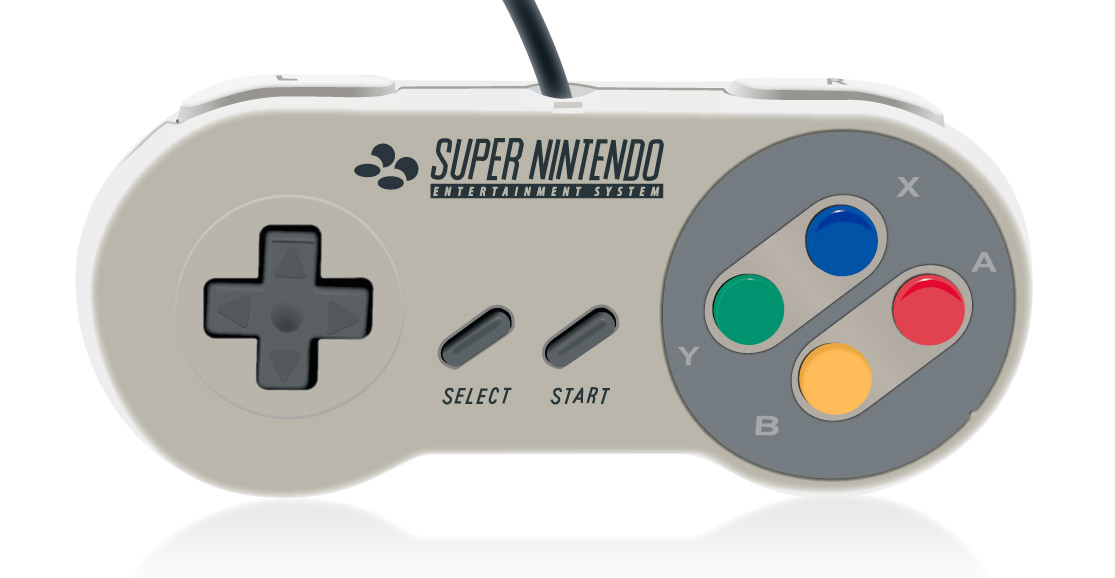
\includegraphics[scale=0.25,clip=true,trim=75 80 75 60]{config_chapter/snes_controller.jpg}
\caption{The original SNES controller. The L (left) and R (right) shoulder buttons are located on the top edge of the controller.}\label{fig:snes_controller}
\end{figure}

As a reference, the original SNES controller is shown in Figure~\ref{fig:snes_controller}.  This controller has a directional pad that provides two "axes" for directional input (an up/down axis and a left-right axis).  It also provides a total of eight buttons: the rectangular start and select buttons, four round input buttons for A/B/X/Y, and two shoulder buttons on the edge of the controller for L (left) and R (right).

BeagleSNES uses the configuration file \texttt{snes9x.conf} to define the \emph{default} mappings between physical joystick buttons and axes to the logical buttons and axes used by the emulator.  \texttt{snes9x.conf} is located in the \texttt{beaglesnes} directory of the \texttt{/boot} partition.  The button mapping settings are located in a section within the \texttt{snes9x.conf} named \texttt{[BeagleSNES Controls]}.  Previous versions of BeagleSNES required users to change this section to map SNES gamepad buttons to the buttons of your joystick.  But, the \texttt{snes9x.conf} configuration file is now completely ''off-limits'' for the end-user.  All button mappings are now set using the \texttt{games.xml} file.

\begin{updateWarn}
Don't touch the \texttt{snes9x.conf} file!  All configuration settings are now made via the \texttt{games.xml} file.
\end{updateWarn}    

The \texttt{<player1>} and \texttt{<player2>} tags in the \texttt{games.xml} file describe button mappings between your joystick and the SNES gamepad. Figure~\ref{fig:controller_map} demonstrates the use of these tags.  The default button mappings are used for any controller or button not explicitly mentioned in the \texttt{games.xml}.  The only exception to this is the \texttt{<pause>} tag.  If you have a joystick with enough buttons to map all of the SNES controller buttons and still have at least one button to spare, the extra button can be mapped to trigger the pause menu.  Unless the \texttt{<pause>} is explicitly mapped, though, no default is mapped.  

\begin{figure}[h]
\begin{verbatim}<?xml version="1.0"?>
<config>
<player1>
  <vaxis>1</vaxis>
  <haxis>0</haxis>
  <L>4</L>
  <R>5</R>
  <A>1</A>
  <B>2</B>
  <X>0</X>
  <Y>3</Y>
  <select>8</select>
  <start>9</start>
  <pause>11</pause>
</player1>
<player 2>
  ... similar tags go here for the player 2 controller ...
</player2>
... other tags go here ...
</config>\end{verbatim}
\caption{Controller button mapping portion of the \texttt{games.xml} file.}\label{fig:controller_map}
\end{figure}

\subsection{Configuring A Pause Combination}\index{Configuring A Pause Combination}\label{sec:conf_pause}

If you can't spare an extra button to trigger the pause menu, you can map the pause to a combination of buttons. When this button combo is pressed on the player 1 controller, the pause menu will trigger.  For example, you can map the left and right trigger buttons and the start and select buttons together as a pause button combo.  When all four are pressed simultaneously, the pause menu triggers.  Because you don't want the pause button combo to be a set of buttons that will interfere with gameplay, selecting three to four buttons for the combo is advised. 

The pause combo is defined by using two tags: \texttt{<pause\_combo>} and \texttt{<pause\_key>}.  An example pause combo that uses the left and right trigger buttons and the start and select buttons is shown in Figure~\ref{fig:pause_combo}.

\begin{figure}[h]
\begin{verbatim}<pause_combo>
  <pause_key>4</pause_key>
  <pause_key>5</pause_key>
  <pause_key>8</pause_key>
  <pause_key>9</pause_key>
</pause_combo>\end{verbatim}
\caption{XML for a pause button combo in the \texttt{games.xml} file.}\label{fig:pause_combo}
\end{figure}

This particular pause combo assumes the same button mapping as seen in the \texttt{<player1>} tag in Figure~\ref{fig:controller_map}.  For example, the first \texttt{<pause\_key>} of the combo is for button \texttt{4}.  The \texttt{<player1>} tag maps \texttt{4} to the left trigger button in the \texttt{<L>} tag. If the button mapping changes in the \texttt{<player1>} tag, the \texttt{<pause\_key>} tags must be changed to match it. 

\subsection{Configuring GPIOs For Input}\index{Configuring GPIOs For Input}\label{sec:config_gpio}

The BBB platform has support for mapping GPIO inputs as player 1 controller inputs.  The SNES directional pad and buttons, and even the pause button, can be mapped to GPIOs.  A maximum of 13 GPIO inputs (four for the d-pad, eight for buttons, and one for pause) can be mapped using a contiguous block of the BBB's pins (P8.7 through P8.19). Mapping the GPIOs uses the \texttt{<gpio>} tag and a series of \texttt{<gpio\_*>} tags that specify particular SNES controller buttons and controls. Figure~\ref{fig:gpio_mapping} shows a sample GPIO mapping.

\begin{figure}[h]
\begin{verbatim}
<gpio>
  <gpio_gpleft>1</gpio_gpleft>
  <gpio_gpright>2</gpio_gpright>
  <gpio_gpup>3</gpio_gpup>
  <gpio_gpdown>4</gpio_gpdown>
  <gpio_L>5</gpio_L>
  <gpio_R>6</gpio_R>
  <gpio_A>7</gpio_A>
  <gpio_B>8</gpio_B>
  <gpio_X>9</gpio_X>
  <gpio_Y>10</gpio_Y>
  <gpio_select>11</gpio_select>
  <gpio_start>12</gpio_start>
  <gpio_pause>13</gpio_pause>
</gpio>\end{verbatim}
\caption{XML for mapping GPIOs to SNES controls in the \texttt{games.xml} file.}\label{fig:gpio_mapping}
\end{figure} 
 
Each individual \texttt{<gpio\_*>} tag contains a number from one through thirteen.  These numbers correspond to the pins on the P8 header of the BBB.  Pin P8.7 is 1, pin P8.8 is 2, etc. up through pin P8.19, which is 13.  If a particular pin number is not mapped, it won't be initialized by BeagleSNES.  For more information on the hardware details of trigger GPIOs for input to BeagleSNES, check out Section~\ref{sec:gpio_hardware}.

\section{Using BeagleSNES}\index{Using BeagleSNES}

Once the system has been configured, it is now ready for use. BeagleSNES expects either one or two USB gamepads to be plugged in.  Two host USB ports on the BB-xM system have been designated by BeagleSNES as the gamepad ports: one for "player one" and the other for "player two".  \emph{Any gamepad that is not plugged into one of these designated USB ports is ignored.} Figure~\ref{fig:bbxm_usb} shows which two BB-xM USB ports are designated for the gamepads. 

\begin{figure}[h]
\centering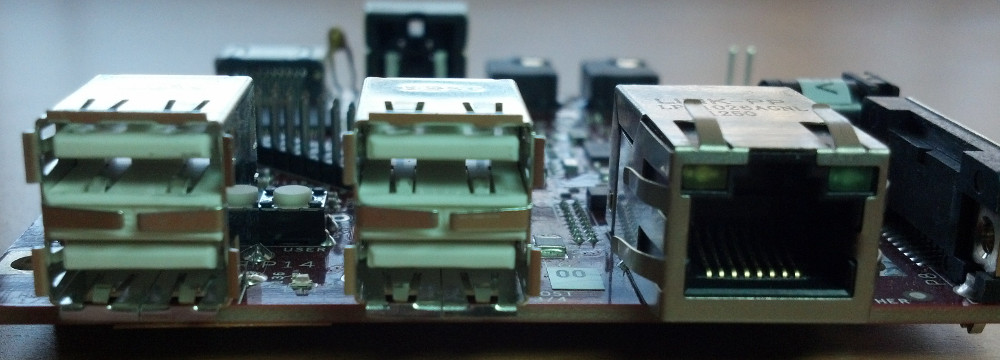
\includegraphics[scale=0.4]{install_chapter/usb_ports.jpg}
\caption{The USB ports of the BB-xM.  The top-left USB port is reserved for the "player one" gamepad, and the top-right USB port is reserved for the "player two" gamepad.}\label{fig:bbxm_usb}
\end{figure}

The BBB has only one host USB port, so there are two options for using gamepads with the system.  The first option is to plug a gamepad into the host USB port.  This is the port for the "player one" gamepad, and no "player two" gamepad can be used.  The second option is to plug a USB hub into the host USB port and then plug one or two gamepads into the hub.  Much like the host USB ports of the BB-xM, one port of the hub will be the "player one" port, and another will be for "player two".  Whichever physical ports on the hub report as the first and second logical ports will be used as the "player one" and "player two" ports, respectively.  \emph{Any gamepad that is not plugged into one of these designated USB ports on the hub is ignored.}

\subsection{Game Selection Menu}\index{Game Selection Menu}\label{sec:game_selection_menu}

Assuming that you have successfully completed the steps of the adding game descriptions, ROMs, and box images to your BeagleSNES system, it will now boot up to a complete menu of SNES titles that are ready to be played.  This game selection menu will \emph{only} respond to the "player one" controller, and the menu will display the text "PLEASE CONNECT PLAYER 1 GAMEPAD" if no gamepad is connected to the "player one" USB port\footnote{The LCD3 display target will not display this warning.}.  Press up and down on the gamepad's direction-pad to change the currently selected title on the menu.  Press either the "select" or "start" gamepad button to launch the currently selected title.  If there are GPIO inputs that are mapped for up/down and start/select, they can also be used to navigate the menu and launch a title. Once a title has been launched, the menu will fade out and the emulator will begin execution.
\begin{updateWarn}
Once you have launched a title and left the game selection menu, you must use the pause menu to return to the game selection menu to select a different game to play.
\end{updateWarn}

\subsection{Pause Menu}\index{Pause Menu}\label{sec:pause_menu}

The pause menu can only be triggered while playing a game.  Its purpose is to allow the user to load and save \emph{snapshots} of the current game state, exit the current game and return to the game selection menu, and, of course, pause the game. Figure~\ref{fig:pause_menu} shows the pause menu.

\begin{figure}[h]
\centering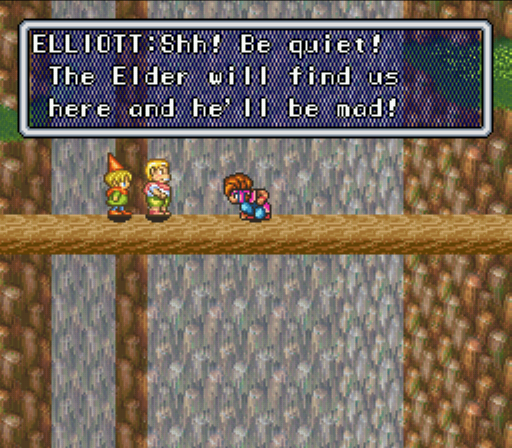
\includegraphics[scale=0.25]{install_chapter/pause1.png} {} 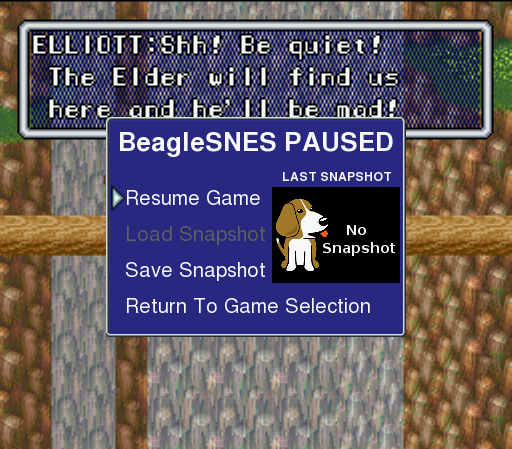
\includegraphics[scale=0.25]{install_chapter/pause2.png} {} 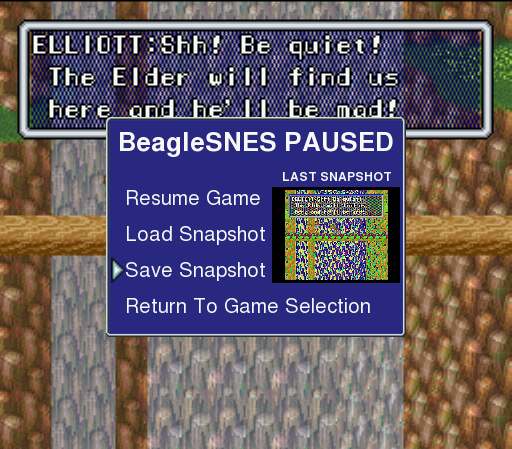
\includegraphics[scale=0.25]{install_chapter/pause3.png}
\caption{The pause menu.  While in-game (left), triggering the pause menu will bring up a set of menu options (middle). If a snapshot for the current game has been previously saved, the ``Load Snapshot'' option will become active and a thumbnail will be shown in the ``LAST SNAPSHOT'' preview window.}\label{fig:pause_menu}
\end{figure}

There are three ways to trigger the pause menu:
\begin{itemize}
\item If the pause menu has been mapped to a single gamepad button in \texttt{games.xml}, press that button. 
\item If a pause button combination has been mapped in \texttt{games.xml}, press that button combo.
\item If the pause menu has been mapped to a GPIO in \texttt{games.xml}, trigger that GPIO.
\end{itemize}

Pressing up and down on the player 1 gamepad, or triggering the appropriate GPIOs, will navigate the pause menu.  Likewise, using select/start or its GPIO equivalent will select a menu option. Selecting ``Resume Game'' will remove the pause menu and unpause the game.  Also, pressing the pause button or button combo, or triggering the pause GPIO, a second time will also remove the pause menu and unpause the game.

The ``Load Snapshot'' and ``Save Snapshot'' menu options allow you to save the current state of the game and then load it to return to it at any time. This is useful for saving the progress of the current play session when you need to take a break and are not near a point in the game where progress can be saved.  It is also useful for saving your game just prior to making that difficult jump or fighting a tough boss battle.  Snapshots are named after the filename of the ROM that they are associated with, so renaming ROMs will make your save states seem to disappear (although they are still present on the microSD card).  If no snapshot for the current game exists, the ``Load Snapshot'' option will be grayed-out and unavailable.  Only one snapshot can exist for each game.  Once a snapshot is saved, the prior snapshot is overwritten.

\begin{updateWarn}
Snapshots are stored in the \texttt{savestate} subdirectory of the \texttt{beaglesnes} directory on the \texttt{/boot} partition.
\end{updateWarn}

The ``Return to Game Selection'' menu option exits the current game and return you to the game selection menu. Be sure to save a snapshot of your current game if you want to return to it later.  Selecting this option is roughly the same as turning off the power on your SNES console: your current game will be lost forever.
  